\documentclass%
%[handout]
{beamer}
% % % % % % % %
% % % % % % % %
% % % % % % % %
%IMPORTANT
%compiles with 
%pdflatex -shell-escape 
%IMPORTANT
% % % % % % % %
% % % % % % % %
% % % % % % % %
\mode<presentation>
{
\useinnertheme{rounded}
\useoutertheme{infolines}
\usecolortheme{orchid}
\usecolortheme{whale}
}

\usepackage[english]{babel}
\usepackage[latin1]{inputenc}
\usepackage[all,cmtip]{xy}
\usepackage{times}
\usepackage[T1]{fontenc}
\usepackage{../example-templates}
\usepackage{../pstricks-commands}
\usepackage{cancel}

\usepackage{auto-pst-pdf}
\usepackage{pst-plot}
%\usepackage{pstricks-add} 

% Or whatever. Note that the encoding and the font should match. If T1
% does not look nice, try deleting the line with the fontenc.

\graphicspath{{../../modules/}}

\newtheoremstyle{partialproof}{3pt}{3pt}{}{}{}{.}{.5em}{}
\theoremstyle{partialproof} \newtheorem{partialproof}[theorem]{Proof.}
%\DeclareMathOperator{\diff}{d}
\newcommand{\diff}{\text{d}}
\setbeamertemplate{navigation symbols}{}

\includeonlylecture{1}

\newcommand{\lect}[3]{
  \date{#1}
  \lecture[#1]{#2}{#3}
}

\setbeamertemplate{footline}
{
  \leavevmode%
  \hbox{%
  \begin{beamercolorbox}[wd=.333333\paperwidth,ht=2.25ex,dp=1ex,center]{author in head/foot}%
    \usebeamerfont{author in head/foot}\insertshortauthor
  \end{beamercolorbox}%
  \begin{beamercolorbox}[wd=.333333\paperwidth,ht=2.25ex,dp=1ex,center]{title in head/foot}%
    \usebeamerfont{title in head/foot}\insertshorttitle
  \end{beamercolorbox}%
  \begin{beamercolorbox}[wd=.333333\paperwidth,ht=2.25ex,dp=1ex,center]{date in head/foot}%
    \usebeamerfont{date in head/foot}\insertshortdate{}
  \end{beamercolorbox}}%
  \vskip0pt%
}

% If you have a file called "university-logo-filename.xxx", where xxx
% is a graphic format that can be processed by latex or pdflatex,
% resp., then you can add a logo as follows:

%\pgfdeclareimage[height=0.8cm]{logo}{bluelogo}
%\logo{\pgfuseimage{logo}}

\begin{document}

\AtBeginLecture{%

\title[\insertlecture]{FreeCalc}
\subtitle{\insertlecture}
\author[FreeCalc]{}
\institute[UMass Boston]{University of Massachusetts Boston}
\date{\insertshortlecture}
\begin{frame}
  \titlepage
\end{frame}
}%

% begin lecture
\lect{\today}{Sample}{1}
%% begin module derivatives-rules-summary
\begin{frame}
\frametitle{Rules of differentiation.}
We studied the basic rules of differentiation.
\begin{itemize}
\item<1->\alert<12>{ $f (g(x))'=f'(g(x)) g'(x) $ (Chain rule). }
\item<2->\alert<12>{ $(f*g)'=f'g+fg'$ (Product rule).}
\item<3->\alert<12>{ $(f+g)'=f'+g'$ (Sum rule). }
\item<4->\alert<12>{ $x'=1$. }
\item<5->\alert<12>{ $(c)'=0$ if $c$ is a constant (Constant derivative rule).}
\end{itemize}
\uncover<6->{We studied additional differentiation rules.}
\begin{itemize}
\item<6->\alert<13>{ $(e^x)'=e^x$ (Exponent derivative rule).}
\item<7->\alert<13>{ $\left(\frac{f}{g}\right)'=\frac{f' g-f g' }{g^2}$ (Quotient rule).}
\item<8->\alert<13>{ $(x^r)'=rx^{r-1} $, $r$-arbitrary real number (Power rule).}
\item<9->\alert<13>{ $(\ln x)'=\frac{1}x$ (Logarithm derivative rule). }
\item<10->\alert<13>{ $(\log_a x)'=\frac{1}{x\ln a}$.}
\item<11->\alert<13>{ $(\sin x)'=\cos x$, $(\cos x)'=-\sin x$}
\end{itemize}

\uncover<12->{We derived \alert<12>{the first set of rules}  by directly computing limits. } \uncover<13->{The \alert<13>{second set of rules} can be derived from the first set \uncover<13>{algebraically}.}
\end{frame}
% end module derivatives-rules-summary

%% begin module power-rule-from-exponent
\begin{frame}
\begin{example}
Let $c$ be a constant. Derive the constant multiple rule 
\[
\alert<6>{(cf)'=c f'}
\]
\uncover<3->{using the \alert<3>{product rule $(fg)'=f'g+fg'$}} \uncover<4->{\alert<4>{and the constant derivative rule $(c)'=0$.}}

\[
\uncover<2->{\alert<3,6>{(cf)'}=} \uncover<3->{\alert<3>{\alert<4>{(c)'} f+ c f'}=}\uncover<4->{\alert<4>{0} f+cf'=}\uncover<5->{\alert<6>{cf'}}
\]
\uncover<6->{\alert<6>{as desired}.}
\end{example}

\end{frame}

%end module power-rule-from-exponent
%% begin module derivatives-rules-relations

\begin{frame}
\begin{example}
Let $n$-positive integer. Derive the positive integer power rules $\left( x^2\right)' =2x$, $\left( x^3\right)' =3x^2$, $\left( x^4\right)' =4x^3$, \dots from the product rule, the sum rule, and the rule $(x)'=1$.

\[
\begin{array}{rcl}
(x)'&=&1\\
\uncover<2->{\alert<4>{(x^2)'}&=& (x*x)'=x'x +x x'= x+x=\alert<4>{2x} } \\
\uncover<3->{\alert<7>{(x^{3})'}&=& (x* x^2)'= x' x^2+x\alert<4>{(x^2)'}= \uncover<4->{x^2+ x (\alert<4>{2x})=}\uncover<5->{x^2+2x^2=\alert<7>{3x^2}}}\\
\uncover<6->{(x^{4})'&=& (x* x^3)'= x' x^3+x\alert<7>{(x^3)'}= \uncover<7->{x^3+ x (\alert<7>{3x^2})=}\uncover<8->{x^3+3x^3=4x^3}}\\
\uncover<9->{&\vdots&}\\ 
\uncover<9->{\alert<11>{(x^{n})'}&=&\dots = \alert<11>{n x^{n-1}}}\\
\uncover<10->{(x^{n+1})'&=& (x*x^n)'=x' x^n+ x\alert<11>{(x^{n})'}=}\uncover<11->{x^n+x (\alert<11>{nx^{n-1}})=}\uncover<12->{(n+1)x^n}\\
\uncover<12->{&\vdots&} 
\end{array}
\]
\end{example}


\end{frame}




%end module derivatives-rules-relations
%% begin module derivatives-rules-relations

\begin{frame}
\begin{example}
Let $n$ be a positive integer. Derive the negative integer power rule
\[
(x^{-n})'=\left(\frac{1}{x^n}\right)'= -n x^{-n-1} =-\frac{n}{x^{n+1}}
\]
\uncover<4->{using \alertNoH{4}{the product rule},} \uncover<5->{\alertNoH{5}{the constant derivative rule}} \uncover<6->{and \alertNoH{6}{the power rule for positive integers}.}

\[
\begin{array}{rcl p{2cm} |r}
\uncover<2->{ x^n x^{-n} &=& 1  &&} \uncover<3->{\frac{\diff}{\diff x}}\\
\uncover<3->{\alertNoH{4}{( x^n x^{-n})'} &=&\alertNoH{5}{(1)'}  }\\

\uncover<4->{ \alertNoH{4}{ \alertNoH{6}{(x^n)'} x^{-n} + x^n (x^{-n})'}&=&\alertNoH{5}{0}}\\
\uncover<6->{ \alertNoH{7}{\alertNoH{6}{n x^{n-1}}x^{-n}}+ x^n (x^{-n})'&=&0 }\\
\uncover<7->{\alertNoH{7}{\frac{n}{x}}+ x^n (x^{-n})'&=&0 }\\
\uncover<8->{x^n (x^{-n})'&=&-\frac{n}x && \frac{1}{x^n}}\\
\uncover<9->{(x^{-n})'&=&-\frac{n}{x^{n+1}}}
\end{array}
\]

\end{example}



\end{frame}




%end module derivatives-rules-relations

%% begin module power-rule-rationa-from-chain-rule
\begin{frame}
\begin{example}
Derive the power rule $\alertNoH{13}{\left(x^{\frac{1}{q}}\right)'=\frac{1}{q} x^{\frac{1}q-1}}$ \uncover<4->{using \alertNoH{4}{the rule $(x)'=1$},} \uncover<6->{\alertNoH{6}{the chain rule}} \uncover<7->{and the \alertNoH{7}{integer power rule $\frac{d}{du}(u^q)=qu^{q-1} $}.}

\[
\begin{array}{rclp{0.3cm}|l}
\uncover<2->{ \left(x^{\frac{1}{q}}\right)^q &=&x&& \uncover<3->{\alertNoH{3}{\frac{d}{dx}}}}\\
\uncover<3->{ \alertNoH{3}{\left(\left(\alertNoH{5}{x^{\frac{1}q}} \right)^q\right)'} &=& \uncover<4->{\alertNoH{4}{1}} \uncover<3>{\alertNoH{3}{(x)'}} &&\uncover<5->{\alertNoH{5,8}{\text{Set~}u=x^{\frac1q} }}}\\
\uncover<5->{ \alertNoH{6}{\left(\alertNoH{5}{u}^{q}\right)'}&=&1  }  \\
\uncover<6->{\alertNoH{6}{ \alertNoH{7}{\frac{d}{du} \left(u^q\right)} u'}&=&1}\\
\uncover<7->{\alertNoH{7}{q (\alertNoH{8}{u})^{q-1}} (\alertNoH{8}{u})'&=&1 }\\
\uncover<8->{ q (\alertNoH{8}{x^{\alertNoH{9}{\frac{1}q}}})^{\alertNoH{9}{q-1}} \left( \alertNoH{8}{x^{\frac1q}}\right)'&=&1 }\\
\uncover<9->{\alertNoH{10}{q x^{\alertNoH{9}{\frac{q-1}q}}}\left( x^{\frac1q}\right)'&=&1&&\uncover<10->{\alertNoH{10}{\text{divide~by~}q x^{\frac{q-1}q}}}}\\
\uncover<10->{\alertNoH{13}{\left( x^{\frac1q}\right)'}&=&\frac{ 1}{\alertNoH{10}{q \alertNoH{11}{x^{\frac{q-1}q}}}}= \uncover<11->{ \frac{\alertNoH{11}{x^{\alertNoH{12}{-\frac{q-1}{q}}}}}{q}=}\uncover<12->{\alertNoH{13}{\frac{1}q x^{\alertNoH{12}{\frac{1}q-1}}}} &&\uncover<13->{\alertNoH{13}{\text{as~desired}}}}
\end{array}
\]
\end{example}

\end{frame}

%end module power-rule-rationa-from-chain-rule

%% begin module quotient-rule-from-power-and-chain
\begin{frame}
\begin{example}
Derive the quotient rules
\[
\begin{array}{rcl}
\alertNoH{5,9}{\displaystyle\left(\frac{1}{g}\right)'}&=&\displaystyle\alertNoH{5,9}{-\frac{g'}{g^2}}
\\
\displaystyle\alertNoH{11}{\left(\frac{f}{g}\right)'}&=&\displaystyle\alertNoH{11}{\frac{f'g-fg'}{g^2}}
\end{array}
\]
\uncover<3->{using \alertNoH{3}{the chain rule},} \uncover<4->{\alertNoH{4}{the negative power rule}} \uncover<8->{and \alertNoH{8}{the product rule}.}
\[
\begin{array}{rclp{0.3cm}|l}
\displaystyle \uncover<2->{ \alertNoH{3,5}{\left(\frac{1}{g}\right)'} &=& \displaystyle \uncover<3->{\alertNoH{3}{\alertNoH{4}{\frac{\diff}{\diff g} \left( \frac1g\right)} g'} =} \uncover<4->{ \alertNoH{5}{\alertNoH{4}{- \frac{1}{ g^2 }}g'}}&&\uncover<5->{\alertNoH{5}{\text{as~desired}}}}\\
\\
\displaystyle
\uncover<6->{\alertNoH{7,11}{\left(\frac{f}{g}\right)'}\uncover<7->{&=&\displaystyle\alertNoH{7,8}{\left( f \frac{1}g\right)'}=}\uncover<8->{\alertNoH{8}{f' \frac{1 }{g} +f\alertNoH{9}{\left( \frac{1}g\right)'}}=}\uncover<9->{ \alertNoH{10}{ \frac{f'}{g} +f\alertNoH{9}{\left(-\frac{g'}{g^2}\right)}}}}\\
\\
\uncover<10->{&=&\displaystyle
%\frac{f'g}{g^2} - \frac{fg'}{g^2}=
\alertNoH{10,11}{\frac{f'g-fg'}{g^2}} &&\uncover<11->{\alertNoH{11}{\text{as~desired}}}}
\end{array}
\]
\end{example}
\end{frame}
%end module quotient-rule-from-power-and-chain

%% begin module power-rule-rationa-from-chain-rule
\begin{frame}
\alert<1>{You will not be tested on the material in the next slide.}
\end{frame}
\begin{frame}

\begin{example}
Derive \alert<11>{the exponent rule $\left(e^x\right)'=e^x$} \uncover<2->{using the Calc II formula below,} \uncover<3->{ \alert<3>{the infinite} {\color{gray!50} (both sides uniformly convergent)} \alert<3>{sum rule $(f_1+f_2 +f_3 +\dots)' =f_1' +f_2'  +f_3' +\dots$}}
\uncover<4->{and \alert<4>{the power rule $(x^n)'=nx^{n-1}$}. } 
\uncover<2->{\[
\alert<2,10>{e^x}=\alert<2,10>{1+x+\frac{x^2}{2!}+\frac{x^3}{3!}+\dots},
\]
}
\uncover<2->{where $n!=1\cdot2\cdot3\cdot \dots\cdot n$.} \uncover<5->{We have that $\alert<5,9>{\frac{n}{\alert<6>{ n!}}} =\uncover<6->{ \frac{\alert<7>{n} }{ \alert<6>{ 1\cdot 2\cdot \dots\cdot (n-1) \cdot  \alert<7>{n}}}=}\uncover<7->{\frac{1}{\alert<8>{1\cdot 2\cdot \dots\cdot (n-1)}}=}\uncover<8->{\alert<9>{ \frac{1}{ \alert<8>{(n-1)!} }}} $.}
\[
\begin{array}{rcl}
\uncover<2->{\alert<11>{\left(\alert<2>{e^x}\right)'} &=&\alert<3>{\left(\alert<2>{1+x+\frac{x^2}{2!}+\frac{x^3}{3!}+\dots} \right)' }} \\
\uncover<3->{&=& \alert<3>{ \alert<4>{(1)'}+\alert<4>{(x)'}+\frac{\alert<4>{(x^2)'}}{2!} +\frac{\alert<4>{(x^3)'}}{3!}+\dots + \frac{\alert<4>{(x^n)'}}{n!}+\dots}}
\\ \uncover<4->{&=&\alert<4>{0}+ \alert<4>{1}+ \frac{\alert<4>{\alert<5-9>{2}x}}{\alert<5-9>{2!}}+ \frac{\alert<4>{\alert<5-9>{3}x^2}}{\alert<5-9>{3!}}+ \dots +\frac{\alert<4>{\alert<5-9>{n}x^{n-1}}}{\alert<5-9>{n!}}+\dots }\\
\uncover<9->{&=& \alert<10>{ \phantom{ 0~ + }  1 + \frac{\phantom{2}x}{\alert<9>{1!}}+\frac{\phantom{3}x^{2}}{\alert<9>{2!}}+\dots+\frac{\phantom{n}x^{n-1}}{\alert<9>{(n-1)!}}+\dots}=}\uncover<10->{\alert<10,11>{e^x}}\\
\end{array}
\]
\uncover<11->{\alert<11>{as desired.}}
\end{example}

\end{frame}

%end module power-rule-rationa-from-chain-rule
%% begin module logarithm-rule-from-exponent
\begin{frame}
\begin{example}
Derive the logarithm derivative rules
\[
\begin{array}{rcl}
\alert<11,15>{(\ln x)'}&=&\alert<11,15>{\frac{1}{x}}\\
\alert<16>{(\log_a x)'}&=&\alert<16>{\frac{1}{x\ln a}}
\end{array}
\]
\uncover<5->{using \alert<5>{the chain rule},} \uncover<6->{the \alert<6>{exponent derivative rule $(e^{x})'=e^x$}, } \uncover<7->{\alert<7>{the rule $(x)'=1$}} \uncover<14->{and the \alert<14>{constant multiple rule $(cf)'=cf'$}.}
\[
\begin{array}{rclp{0.3cm}|l}
\uncover<2->{
e^{\alert<3>{\ln x}}&=&x && \uncover<3->{ \alert<3,8>{ \text{set~~~}u =\ln x }}}\\
\uncover<3->{e^{\alert<3>{u}}&=&x&& \uncover<4->{\alert<4>{\frac{d}{dx}}}}\\
\uncover<5->{ \alert<5>{\alert<6>{\frac{d}{du}(e^u)} u'}&=&\alert<7>{(x)'}}\\
\uncover<6->{ \alert<6>{e^{\alert<8>{u}}} \alert<8>{u}'&=&\alert<7>{1}}\\
\uncover<8->{\alert<9>{e^{\alert<8>{\ln x}}} (\alert<8>{\ln x})'&=&1}\\
\uncover<9->{\alert<9>{x}(\ln x)'&=&1&&\uncover<11->{\alert<11>{\cdot \frac1x}}}\\
\uncover<10->{ \alert<11>{(\ln x)'} &=& \displaystyle\alert<11>{\frac{1}x} & &\uncover<11->{ \alert<11>{ \text{as~desired}}}}\\ \hline 
\uncover<12->{\alert<16>{(\alert<13>{\log_a x})'} & =&  \uncover<13->{\alert<14>{\left(\alert<13>{\frac{\ln x}{\ln a}}\right)' }=} \uncover<14->{\alert<14>{ \frac{ \alert<15>{ (\ln x)'}}{\ln a}} =} \uncover<14->{\alert<16>{ \frac{ \alert<15>{1} }{\alert<15>{x}\ln a}}}& & \uncover<16>{ \alert<16>{ \text{as~desired~}}}}
\end{array}
\]
\end{example}
\end{frame}

%end module module logarithm-rule-from-exponent
%% begin module power-rule-from-exponent
\begin{frame}
\begin{example}

\end{example}

\end{frame}

%end module power-rule-from-exponent
%\input{../../modules/derivatives-computation-understanding/sine-rule-from-exponent}
%\section{Derivatives and the Shapes of Curves}
%\subsection{What Does $f''$ Say About $f$?}
%% begin module concavity-def
\begin{frame}
\frametitle{What Does $f''$ Say About $f$?}
$f$ and $g$ are both increasing functions on $(a,b)$ with the same end points, but they look different because they bend in different directions.
\begin{columns}[c]
\column{.5\textwidth}
\ \only<handout:0| -2>{%
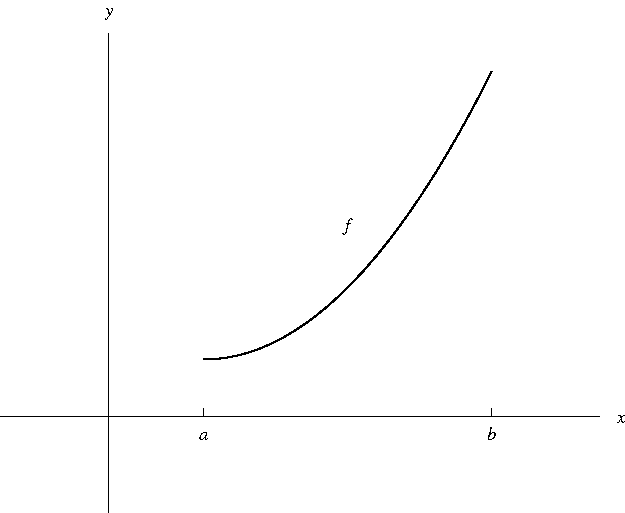
\includegraphics[height=3.5cm]{curve-sketching/pictures/04-03-concaveupa.pdf}%
}%
\only<handout:0| 3>{%
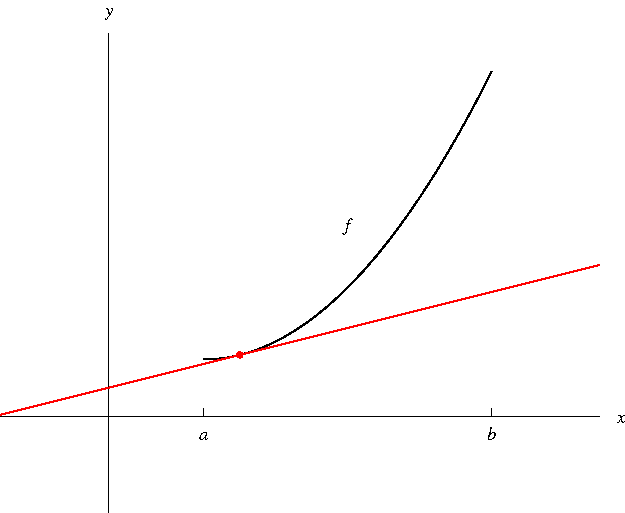
\includegraphics[height=3.5cm]{curve-sketching/pictures/04-03-concaveupb.pdf}%
}%
\only<handout:0| 4>{%
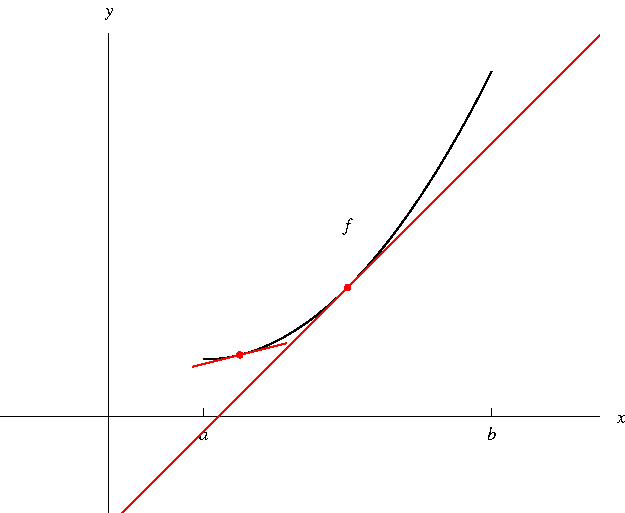
\includegraphics[height=3.5cm]{curve-sketching/pictures/04-03-concaveupc.pdf}%
}%
\only<handout:0| 5>{%
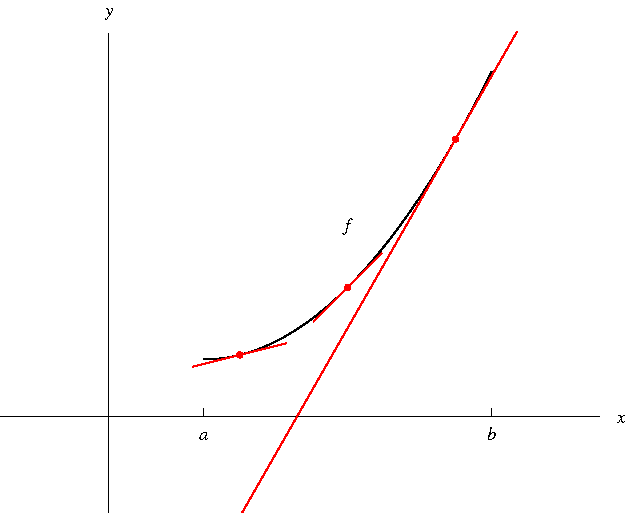
\includegraphics[height=3.5cm]{curve-sketching/pictures/04-03-concaveupd.pdf}%
}%
\only<6->{%
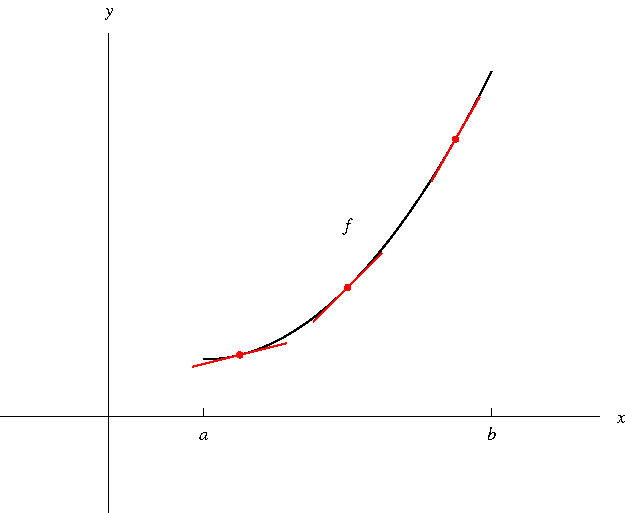
\includegraphics[height=3.5cm]{curve-sketching/pictures/04-03-concaveupe.pdf}%
}%

%\begin{center}
\ \ \ \ \ \ \ \ \ \uncover<6->{Concave up}
%\end{center}
\column{.5\textwidth}
\ \only<handout:0| -2>{%
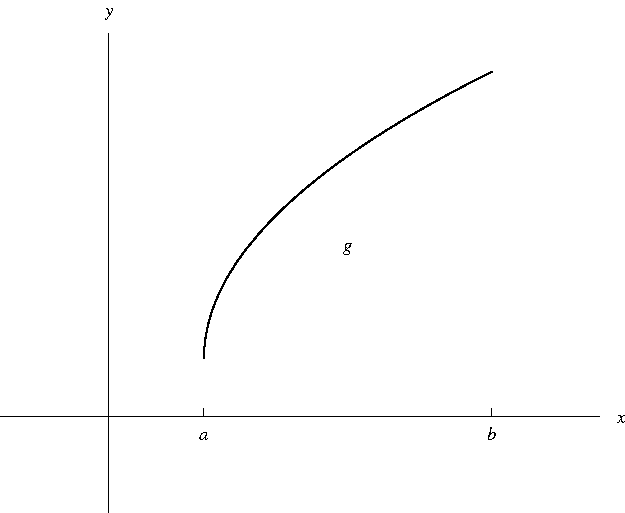
\includegraphics[height=3.5cm]{curve-sketching/pictures/04-03-concavedowna.pdf}%
}%
\only<handout:0| 3>{%
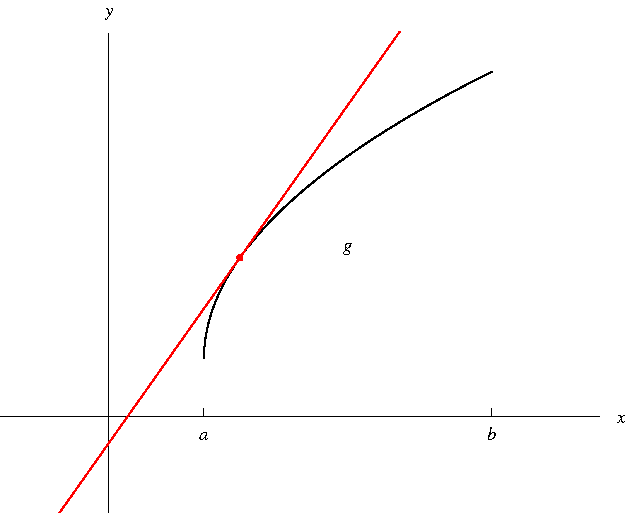
\includegraphics[height=3.5cm]{curve-sketching/pictures/04-03-concavedownb.pdf}%
}%
\only<handout:0| 4>{%
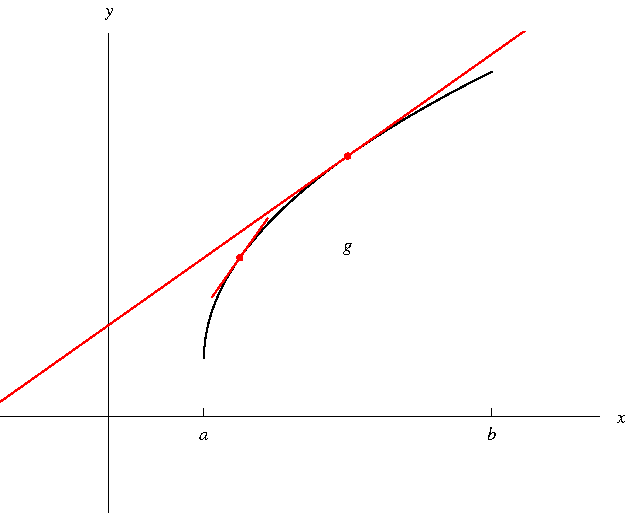
\includegraphics[height=3.5cm]{curve-sketching/pictures/04-03-concavedownc.pdf}%
}%
\only<handout:0| 5>{%
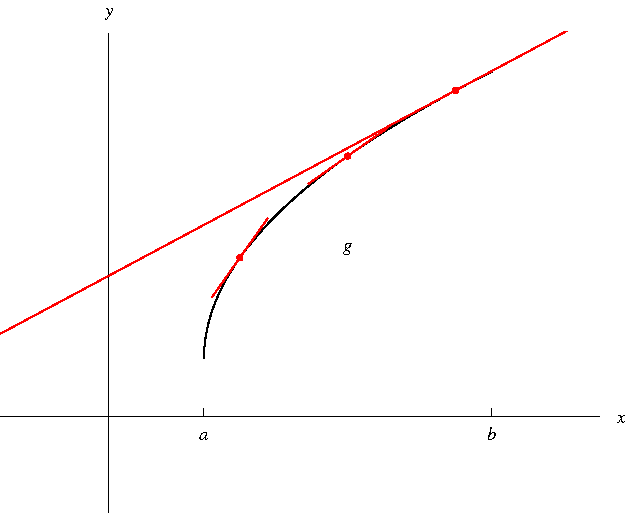
\includegraphics[height=3.5cm]{curve-sketching/pictures/04-03-concavedownd.pdf}%
}%
\only<6->{%
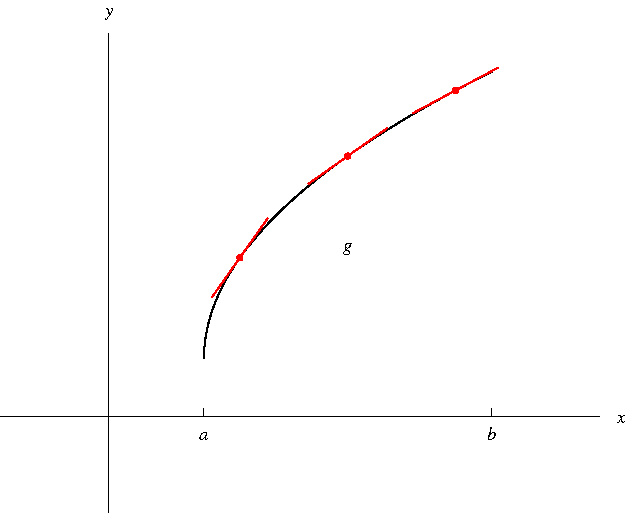
\includegraphics[height=3.5cm]{curve-sketching/pictures/04-03-concavedowne.pdf}%
}%

%\begin{center}
\ \ \ \ \ \ \ \ \ \uncover<6->{Concave down}
%\end{center}
\end{columns}
\uncover<2->{%
\begin{definition}[Concave Up/Concave Down]
Let $f$ be a differentiable function.  If the graph of $f$ lies above all of its tangents on an interval $I$, then it is called concave up on $I$.  If it lies below all of its tangents on $I$, it is called concave down on $I$.
\end{definition}
}%
\end{frame}
% end module concavity-def

%% begin module second-derivative-test
\begin{frame}
This gives us a new way of checking if critical points are local maxima or local minima:

\vspace{.3in}

The Second Derivative Test

Suppose $f''$ is exists near $c$.
\begin{enumerate}
\item  If $f'(c) = 0$ and $f''(c) > 0$, then $f$ has a local minimum at $c$.
\item  If $f'(c) = 0$ and $f''(c) < 0$, then $f$ has a local maximum at $c$.
\end{enumerate}
\uncover<2->{%
\begin{columns}[c]
\column{.3\textwidth}
\psset{xunit=1cm, yunit=1cm}
\begin{pspicture}(-0.5,-0.5)(3.3,2.6)
\tiny
\psaxes[ticks=none, labels=none]{<->}(0,0)(-0.5,-0.5)(3.3,2.6)
\fcLabels{3.3}{2.6}
%Function formula: -5/2-2 ((x) (x))+6 (x)
\psplot[linecolor=red, plotpoints=1000]{0.381966011}{2.618033989}{x 6 mul x x mul -2 mul add -2.5 add }
\psline[linestyle=dashed](1.5, 2)(1.5, 0)
\fcFullDot{1.5}{2}
\psline[linecolor=\fcColorTangent](-0.1,2)(2.9,2)
\tiny
\rput[t](1.5, -0.1){$c$}
\end{pspicture}

%\ 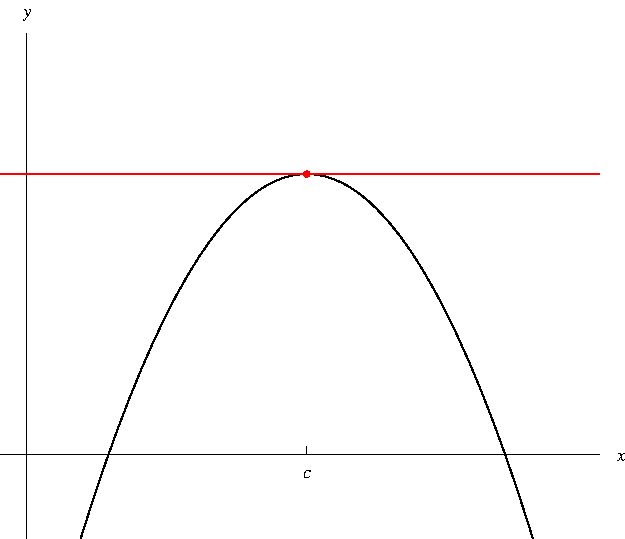
\includegraphics[height=3.5cm]{curve-sketching/pictures/04-03-secondderiv.pdf}%
\column{.7\textwidth}
\begin{itemize}
\item  $f'(c) = 0$, so $f$ has a horizontal tangent at $c$.
\item  $f''(c) < 0$, so $f$ is concave down near $c$.
\item  This means $f$ lies below its horizontal tangent.
\item  This means $f(c)$ is a local maximum.
\end{itemize}
\end{columns}
}%
\end{frame}
% end module second-derivative-test

%% begin module curve-sketching-ex6
\begin{frame}
\begin{example}
Discuss the curve $y = \alert<handout:0| 19-20,39-42>{f(x)}$ \alert<handout:0| 19-20,39-42>{$= x^4 - 4x^3$} with respect to \alert<handout:0| 28-35>{concavity}, \alert<handout:0| 36-42>{points of inflection}, and \alert<handout:0| 10-27>{local maxima and minima}.  \alert<handout:0| 43->{Sketch the curve.}
\begin{columns}[c]
\column{.42\textwidth}
\psset{xunit=0.8cm, yunit=0.1cm}
\begin{pspicture}(-1.1, -5)(4.1,5) 
\psframe*[linecolor=white](-1.2,-32)(4.3,10) 
\tiny 
\psaxes[ticks=none, labels=none]{<->}(0,0)(-1.2,-30)(4.3,9)
\psLabels{4.3}{9}
\psYTickWithLabel{-10}{$-10$}
\psYTickWithLabel{-20}{$-20$}
\psYTickWithLabel{-30}{$-30$}
\psline(1, -0.8)(1,0.8)
\psline(2, -0.8)(2,0.8)
\psline(3, -0.8)(3,0.8)
\rput[t](1, -1.6){$1$}
\rput[t](2, -1.6){$2$}
\rput[t](3, -1.6){$3$}

%Function formula: (x)^{4}-4 ((x)^{3}) 
\rput(2,5){$y=x^{4}-4 x^{3}$} 
\uncover<44->{
\psplot[linecolor=\psColorGraph, plotpoints=1000] {-1.1} {0} {x 3 exp -4 mul x 4 exp add }
}
\uncover<46->{
\psplot[linecolor=\psColorGraph, plotpoints=1000] {0} {2} {x 3 exp -4 mul x 4 exp add }
}
\uncover<48->{
\psplot[linecolor=\psColorGraph, plotpoints=1000] {2} {4.1} {x 3 exp -4 mul x 4 exp add }
}
\uncover<20->{
\psFullDot{3}{-27}
\rput[tr](2.8, -27.5){$(3, -27)$}
}
\uncover<40->{\psFullDot{0}{0}
\psFullDot{0}{0}
\rput[tr](-0.2, -0.5){$(0, 0)$}
}
\uncover<42->{
\psFullDot{2}{-16}
\rput[tr](1.8, -16.5){$(2, -16)$}
}
\end{pspicture} 

%\ \only<handout:0| -19>{%
%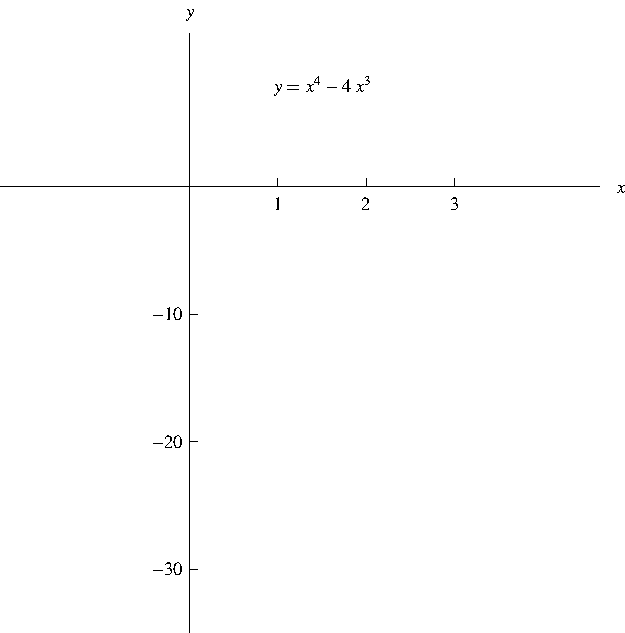
\includegraphics[height=4.5cm]{curve-sketching/pictures/04-03-ex6a.pdf}%
%}%
%\only<handout:0| 20-39>{%
%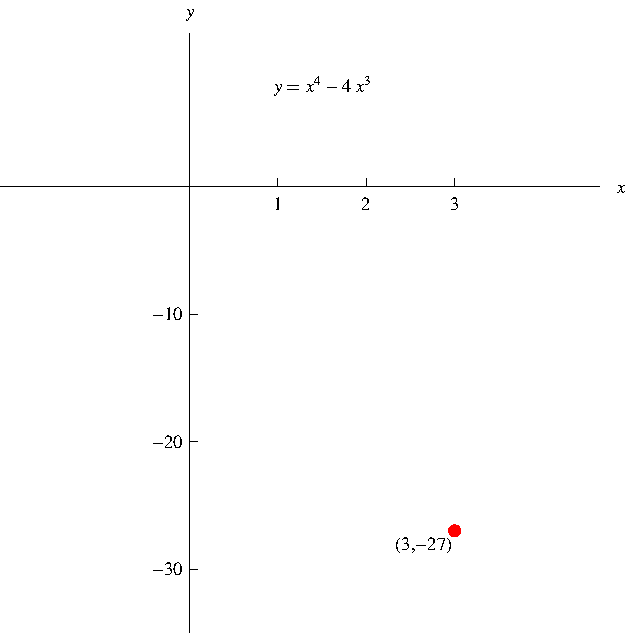
\includegraphics[height=4.5cm]{curve-sketching/pictures/04-03-ex6b.pdf}%
%}%
%\only<handout:0| 40-41>{%
%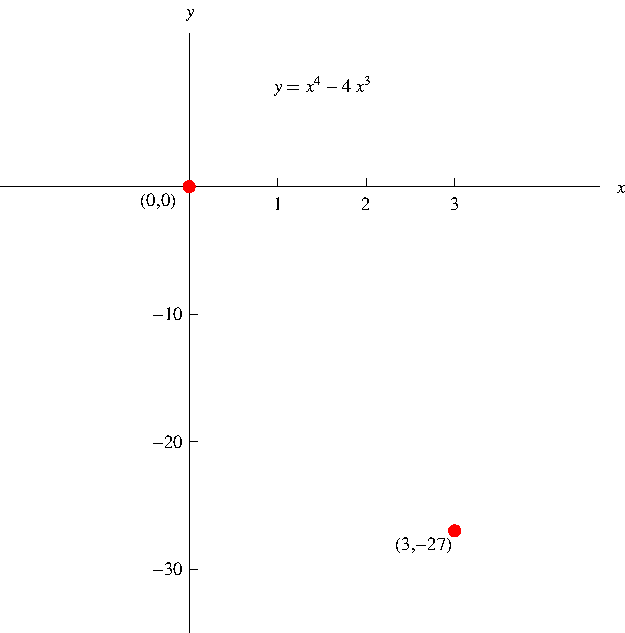
\includegraphics[height=4.5cm]{curve-sketching/pictures/04-03-ex6c.pdf}%
%}%
%\only<handout:0| 42-43>{%
%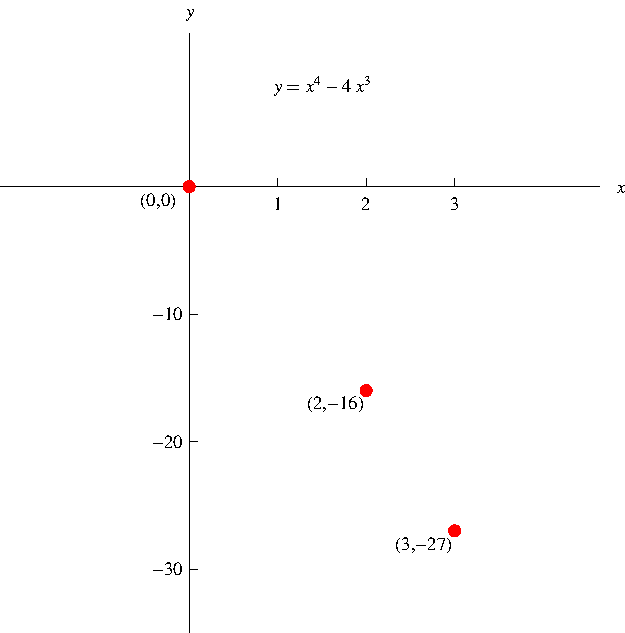
\includegraphics[height=4.5cm]{curve-sketching/pictures/04-03-ex6d.pdf}%
%}%
%\only<handout:0| 44-45>{%
%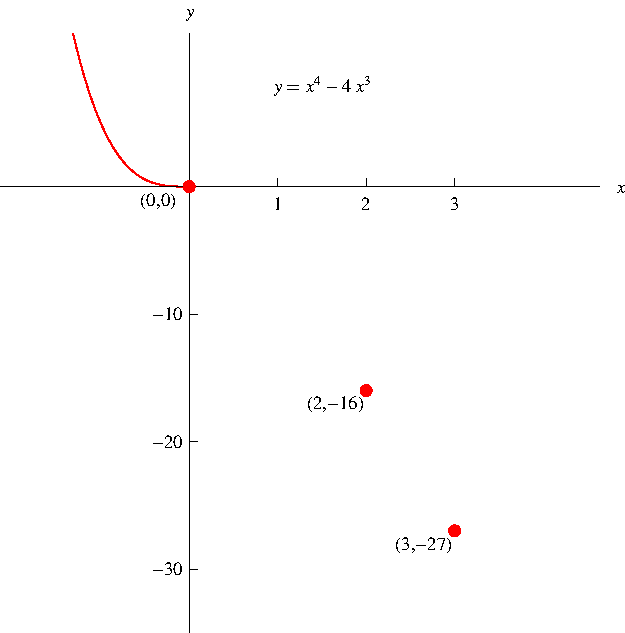
\includegraphics[height=4.5cm]{curve-sketching/pictures/04-03-ex6e.pdf}%
%}%
%\only<handout:0| 46-47>{%
%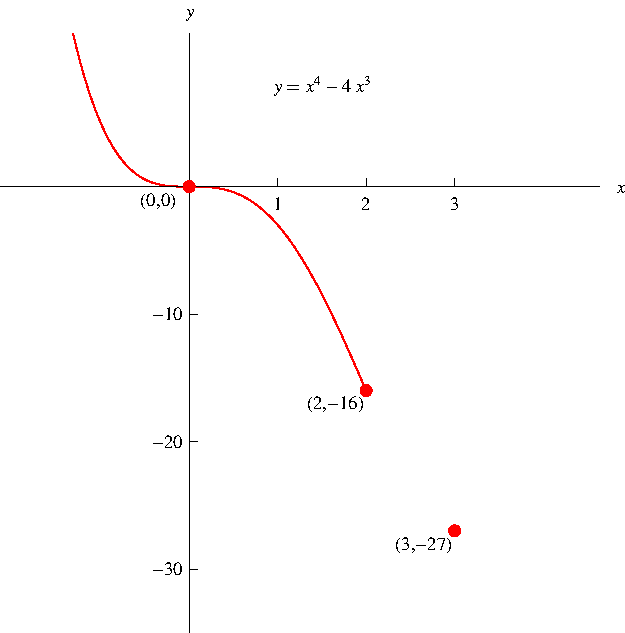
\includegraphics[height=4.5cm]{curve-sketching/pictures/04-03-ex6f.pdf}%
%}%
%\only<48->{%
%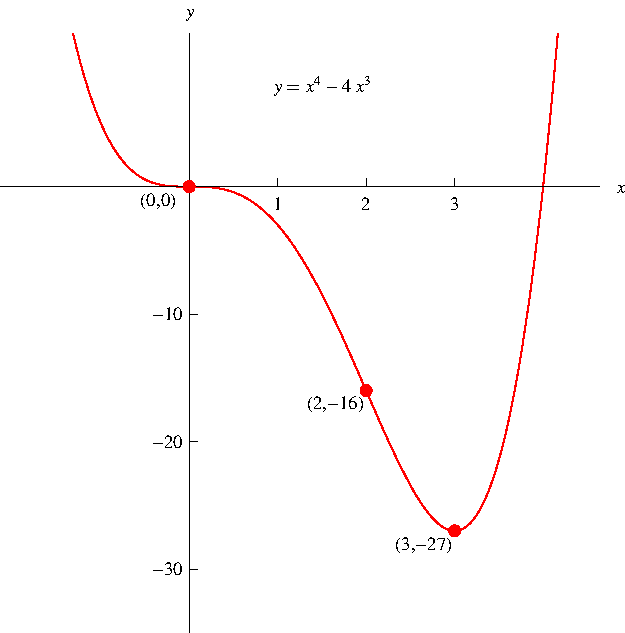
\includegraphics[height=4.5cm]{curve-sketching/pictures/04-03-ex6g.pdf}%
%}%

\vspace{.1in}

\uncover<28->{%
\ \ \ \begin{tabular}{|@{\ }r@{\ }|@{\ }c@{\ }|@{\ }l@{\ }|}
\hline
Interval & $f''(x)$ & \alert<handout:0| 35,43-48>{Concave}\\
\hline
\alert<handout:0| 29-30,37,43-44>{$(-\infty , 0)$} &%
\uncover<30->{\alert<handout:0| 30,37>{$+$}} &%
\uncover<35->{\alert<handout:0| 35,43-44>{up}}\\
\alert<handout:0| 31-32,37-38,45-46>{$(0, 2)$} &%
\uncover<32->{\alert<handout:0| 32,37-38>{$-$}} &%
\uncover<35->{\alert<handout:0| 35,45-46>{down}}\\
\alert<handout:0| 33-34,38,47-48>{$(2, \infty )$} &%
\uncover<34->{\alert<handout:0| 34,38>{$+$}} &%
\uncover<35->{\alert<handout:0| 35,47-48>{up}}\\
\hline
\end{tabular}
}%
\column{.58\textwidth}
\begin{itemize}
\item<2-| alert@2-3,23-26>  $f'(x) = $ \alert<handout:0| 4-5>{\uncover<3->{$4x^3 - 12x^2$} \uncover<4->{$ = $}\uncover<5->{$4\alert<handout:0| 11>{x^2}\alert<handout:0| 12>{(x-3)}$.}}
\item<2-| alert@6-7,29-34>  \alert<handout:0| 13-16>{$f''(x) = $} \alert<handout:0| 8-9>{\uncover<7->{\alert<handout:0| 13-16>{$12x^2 - 24x$}} \uncover<8->{$ = $} \uncover<9->{$12x(x-2)$.}}
\item<10->  Critical numbers: \uncover<11->{\alert<handout:0| 11,21-22>{$0$}} and \uncover<12->{\alert<handout:0| 12,17-18>{$3$}.}
\item<13->  \alert<handout:0| 13-14,21-22>{$f''(0) = \uncover<14->{0}$} and \alert<handout:0| 15-18>{$f''(3) =$ \uncover<16->{$36 > 0$.}}
\item<17->  Second Derivative Test:
\item<17-| alert@17-18>  \alert<handout:0| 47-48>{Local \uncover<18->{minimum} at $3$.}  \alert<handout:0| 19-20>{\uncover<19->{$f(3) =$ \uncover<20->{$-27$.}}}
\item<22-| alert@22>  No information about $0$.
\item<23->  First Derivative Test:
\item<23->  \alert<handout:0| 23-24>{$f'$ is \uncover<24->{$-$} on $(-\infty , 0)$} \alert<handout:0| 25-26>{and \uncover<26->{$-$} on $(0, 3)$}.
\item<27->  No local max or min at $0$.
\item<36->  Inflection points: \alert<handout:0| 39-40>{$\uncover<39->{(}\uncover<37->{\alert<handout:0| 37>{0}}\uncover<39->{,\uncover<40->{0})}$} and \alert<handout:0| 41-42>{$\uncover<39->{(}\uncover<38->{\alert<handout:0| 38>{2}}\uncover<39->{,\uncover<42->{-16})}$}
\end{itemize}
\end{columns}
\end{example}
\end{frame}
% end module curve-sketching-ex6

%% begin module differentiation-formulas-ex1
\begin{frame}
\alert<1>{You will not be tested on the material in the following slide.}
\end{frame}
\begin{frame}
\frametitle{Derivative ball volume =surface area}
The relationship between surface area and volume of a ball.

\footnotesize
\begin{tabular}{|p{0.7cm}p{2cm}p{1cm}p{1cm}p{1cm}p{1cm}p{2.5cm}|}\hline
\alert<0>{Di-men-sion} & \alert<2,14,26>{Pts. at distance $\leq r$ from origin} &  \alert<4,16,28>{Inside-volume name} & \alert<6, 18,30>{Inside-volume f-la} & \alert<8,20,32>{Boundary name} & \alert<10,22,34>{Boundary area f-la} & \alert<12,24,36>{Derivative inside-volume}\\\hline
%
\alert<2>{3} & \uncover<3->{\alert<3>{ball}} & \uncover<5->{\alert<5>{ball volume}} &  \uncover<7->{\alert<7, 12>{$\frac {4}{3}\pi r^3$}} & \uncover<9->{\alert<9>{sphere surface area} } & \uncover<11->{\alert<11, 13>{$4\pi r^2$}} & \uncover<12->{$\alert<12>{\frac{d}{dr}\left(\frac {4}{3}\pi r^3\right)=}\uncover<13->{\alert<13>{4\pi r^2}}$} \\\hline
%
\alert<14>{2} & \uncover<15->{\alert<15>{disk, circle}} & \uncover<17->{\alert<17>{circle area}} & \uncover<19->{\alert<19,24>{$\pi r^2$}} & \uncover<21->{\alert<21>{circle circum-ference}} & \uncover<23->{\alert<23,25>{$2\pi r$}} & \uncover<24->{${\alert<24>{\frac{d}{dr}\left(\pi r^2\right)=}} \uncover<25->{\alert<25>{2\pi r}}$} \\\hline
%
\alert<26>{1} & \uncover<27->{\alert<27>{interval}} & \uncover<29->{\alert<29>{length}} & \uncover<31->{\alert<31>{$2r$}} & \uncover<33->{\alert<33>{the two endpoints}} & \uncover<35->{\alert<35,37>{$2$}} &\uncover<36->{$\alert<36>{\frac{d}{dr}(2r)=} \uncover<37->{\alert<37>{2}}$} \\
\hline
\end{tabular}
\end{frame}
% end module differentiation-formulas-ex1

%% begin module differentiable-ex5
\begin{frame}
\begin{example}[Example 6, p. 150]
Where is the function $f(x) = |x|$ differentiable?
\begin{columns}[c]
\column{.25\textwidth}
\ 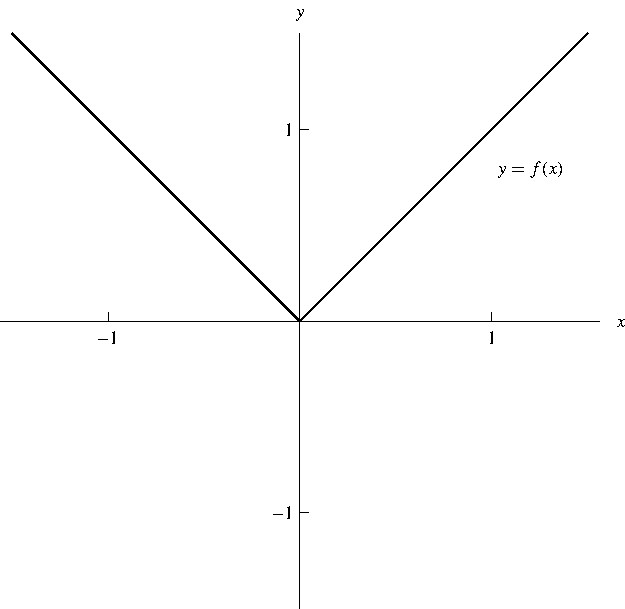
\includegraphics[height=3cm]{derivatives/pictures/03-02-ex5a.pdf}%

\ \only<handout:-2| -30>{%
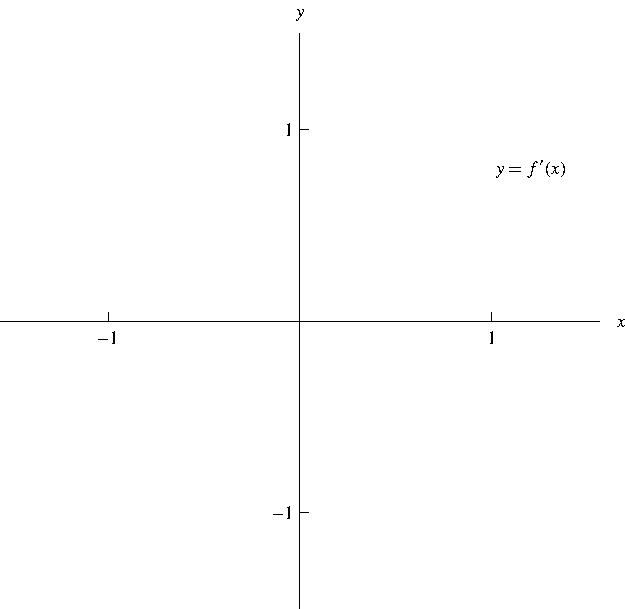
\includegraphics[height=3cm]{derivatives/pictures/03-02-ex5b.pdf}%
}%
\only<handout:3| 31->{%
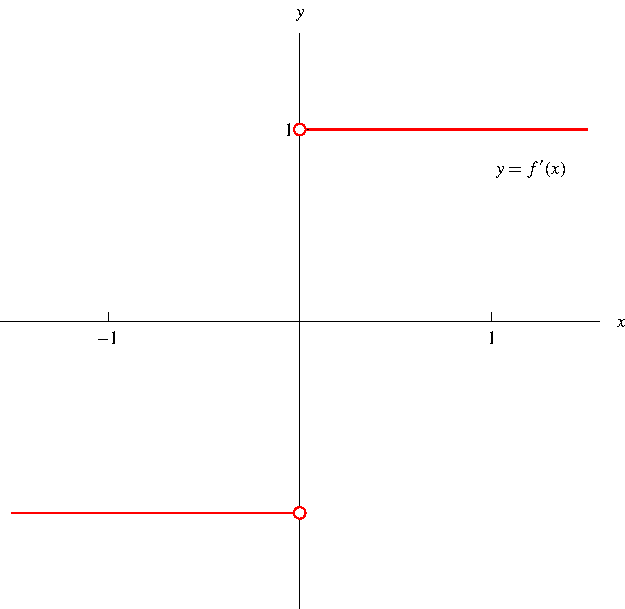
\includegraphics[height=3cm]{derivatives/pictures/03-02-ex5c.pdf}%
}%
\column{.75\textwidth}
\only<handout:1| -10>{%
\begin{itemize}
\item<2->  Suppose $x > 0$.
\item<3-| alert@7>  Then $|x| = x$.
\item<4->  Pick $h$ small so that $x + h > 0$.
\item<5-| alert@7>  Then $|x + h| = x+h$.
\end{itemize}
\abovedisplayskip=0pt
\belowdisplayskip=0pt
\begin{align*}
\uncover<6->{f'(x)}%
 & \uncover<6->{ = } %
\uncover<6->{\lim_{h\rightarrow 0} \frac{|x+h|-|x|}{h}}\\%
 & \uncover<7->{ = } %
\uncover<7->{\lim_{h\rightarrow 0} \frac{(x+h)-x}{h}}\\%
 & \uncover<8->{ = } %
\uncover<8->{\lim_{h\rightarrow 0} \frac{h}{h}}\uncover<9->{ = 1}%
\end{align*}
\uncover<10->{%
Therefore $f$ is differentiable for any $x > 0$.
}%
}%

\only<handout:2| 11-19>{%
\begin{itemize}
\item<11->  Suppose $x < 0$.
\item<12-| alert@16>  Then $|x| = -x$.
\item<13->  Pick $h$ small so that $x + h < 0$.
\item<14-| alert@16>  Then $|x + h| = -(x+h)$.
\end{itemize}
\abovedisplayskip=0pt
\belowdisplayskip=0pt
\begin{align*}
\uncover<15->{f'(x)}%
 & \uncover<15->{ = } %
\uncover<15->{\lim_{h\rightarrow 0} \frac{|x+h|-|x|}{h}}\\%
 & \uncover<16->{ = } %
\uncover<16->{\lim_{h\rightarrow 0} \frac{-(x+h)+x}{h}}\\%
 & \uncover<17->{ = } %
\uncover<17->{\lim_{h\rightarrow 0} \frac{-h}{h}}\uncover<18->{ = -1}%
\end{align*}
\uncover<19->{%
Therefore $f$ is differentiable for any $x < 0$.
}%
}%


\only<handout:3| 20->{%
If $f'(0)$ exists, then 
\[
f'(0) = \lim_{h\rightarrow 0}\frac{f(0+h) - f(0)}{h} = \lim_{h\rightarrow 0} \frac{|0+h| - |0|}{h}.
\]
\uncover<21->{%
Does this limit exist?
}%
\abovedisplayskip=0pt
\belowdisplayskip=0pt
\[
\uncover<22->{%
\lim_{h\rightarrow 0^{\alert<handout:0| 24>{+}}}\frac{|0+h|-|0|}{h}
}%
\uncover<23->{%
 = \lim_{h\rightarrow 0^{\alert<handout:0| 24>{+}}}\frac{\alert<handout:0| 24>{|h|}}{h}
}%
\uncover<24->{%
 = \lim_{h\rightarrow 0^{\alert<handout:0| 24>{+}}}\frac{\alert<handout:0| 24>{h}}{h}
}%
\uncover<25->{%
 = 1
}%
\]
\abovedisplayskip=0pt
\belowdisplayskip=0pt
\[
\uncover<26->{%
\lim_{h\rightarrow 0^{\alert<handout:0| 28>{-}}}\frac{|0+h|-|0|}{h}
}%
\uncover<27->{%
 = \lim_{h\rightarrow 0^{\alert<handout:0| 28>{-}}}\frac{\alert<handout:0| 28>{|h|}}{h}
}%
\uncover<28->{%
 = \lim_{h\rightarrow 0^{\alert<handout:0| 28>{-}}}\frac{\alert<handout:0| 28>{-h}}{h}
}%
\uncover<29->{%
 = -1
}%
\]
\uncover<30->{%
Therefore $f$ is not differentiable at $0$.
}%
\uncover<31->{%
\abovedisplayskip=0pt
\belowdisplayskip=0pt
\[
f'(x) = \left\{ \begin{array}{rl}
1 & \textrm{ if } x > 0\\
-1 & \textrm{ if } x < 0\\
\end{array}\right.
\]
}%
}%
\end{columns}
\end{example}
\end{frame}
% end module differentiable-ex5

%% begin module chain-rule-statement
\begin{frame}
\begin{theorem}[Chain rule]
Let \alert<6,11,12>{$g$-differentiable at neighborhood of $a$}, \alert<9,13>{$f$-diff. at neighb. of $g(a)$}.
\[
\alert<14>{  \alert<3>{\left(f(g(x))\right)'_{|x=a}}= f'(g(a)) g'(a)}
\]
\end{theorem}
\begin{proof}[Proof with \alert<2>{additional assumptions} -motivation for actual proof]
\uncover<2->{
\alert<2>{Suppose that \alert<5>{$g(x)\neq g(a)$ so long as $x\neq a$}}.  \uncover<8->{\alert<8>{Set $G(y)=\frac{f(y)-f(g(a))}{y-g(a)}$.}} \uncover<9->{\alert<9>{ $G(y)$ is continuous at $g(a)$} $\Rightarrow$} \uncover<10->{\alert<10>{$G(g(x))$ is continuous at $a$.}} \uncover<12->{\alert<12>{Furthermore $g(x)$ is continuous at $a$.}}

$\begin{array}{rcl}
\uncover<3->{\alert<14>{ \alert<3>{(f \circ g)'(a)}} &=& \uncover<4->{\displaystyle\lim_{x\to a} \frac{f(g(x)) - f(g(a)) }{x-a}} }\\
\uncover<5->{&=&\displaystyle \alert<6,7>{ \lim_{x\to a} } \alert<7>{\left(\frac{f(g(x)) - f(g(a)) }{\alert<5>{g(x)-g(a)}}\right)} \alert<6>{ \left(\frac{ \alert<5>{ g(x)-g(a)} }{x-a}\right)} }\\
\uncover<6->{&=&\displaystyle \alert<7-10>{\lim_{x\to a}\left( \frac{f(\alert<12>{g(x)}) - f(g(a)) }{\alert<12>{g(x)}-g(a)}\right)}  \alert<6,11>{\lim_{x\to a}\left(\frac{g(x)-g(a)}{x-a}\right)} }\\
\uncover<11->{&=&\displaystyle \alert<13>{\left(\lim_{\alert<12>{y=g(x),y\to g(a)}} \frac{f(\alert<12>{y}) - f(g(a)) }{\alert<12>{y}-g(a)}\right) } \alert<11>{g'(a)}=\uncover<13->{\alert<14>{ \alert<13>{f'(g(a))}g'(a)}}\quad .}
\end{array}
$
}
\end{proof}
\end{frame}
% end module chain-rule-statement

%% begin module chain-rule-statement
\begin{frame}
\begin{theorem}[Chain rule]
\alertNoH{17}{$g$-diff. near $a$}, \alertNoH{4}{$f$-diff. near $g(a)$} $\Rightarrow$ $\alertNoH{18}{ \left(f(g(a))\right)'= f'(g(a)) g'(a)}$ .
\end{theorem}
\begin{proof}
\uncover<2->{Define $Q(\alertNoH{8}{y})=\left\{\begin{array}{ll}\alertNoH{4}{\frac{f(\alertNoH{8}{y})-f(g(a))}{\alertNoH{3}{\alertNoH{8}{y}-g(a)}}, }&\alertNoH{4}{\alertNoH{3}{\alertNoH{8}{y}\neq g(a)}} \\\alertNoH{5}{f'(g(a)), } &\alertNoH{5}{\alertNoH{8}{y}=g(a)} \end{array} \right.$.} \uncover<3->{\alertNoH{3,6}{$Q(g(x))$ - defined for all $x$ near $a$.}}
\uncover<4->{Therefore $\alertNoH{4,5,16}{f'(g(a))}\alertNoH{4,5}{=\lim_{y\to a} Q(y)}\alertNoH{6}{= \alertNoH{16}{\lim_{x\to a} Q(g(x))}}$. }
~\\~\\

$\begin{array}{rcl}
\uncover<7->{\alertNoH{14}{ Q(\alertNoH{8}{g(x)})\frac{g(x)-g(a)}{x-a}} &=&}\uncover<8->{ \left\{\begin{array}{ll} \frac{\alertNoH{11}{(f(\alertNoH{8}{g(x)})-f(g(a))) }} {\alertNoH{10}{(\alertNoH{8}{g(x)}-g(a))}} \frac{\alertNoH{10}{(g(x)-g(a))}}{\alertNoH{11}{x-a}} , &\alertNoH{8}{g(x)}\neq g(a) \\ f'(\alertNoH{8}{g(a)})\frac{\alertNoH{9}{\alertNoH{8}{g(a)}-g(a)}}{x-a}\uncover<9->{\alertNoH{9}{=0}}, & \alertNoH{8}{g(x)}=g(a) \end{array} \right. }\\\uncover<10->{ &=&\alertNoH{11,14}{\frac{f(g(x))-f(a)}{x-a}.}}
\end{array}
$
~\\~\\~\\

$\begin{array}{rcl}
\uncover<12->{\alertNoH{18}{ (f \circ g)'(a)} &=&} \uncover<13->{\displaystyle\lim_{x\to a} \alertNoH{14}{\frac{f(g(x)) - f(g(a)) }{x-a}}=} \uncover<14->{\lim_{x\to a} \alertNoH{14}{Q(g(x)) \frac{g(x)-g(a)}{x-a}}}\\
\uncover<15->{&=&\alertNoH{16}{\displaystyle \lim_{x\to a} Q(g(x))}\alertNoH{17}{\lim_{x\to a} \frac{g(x)-g(a)}{x-a}}} \uncover<16->{=\alertNoH{18}{ \alertNoH{16}{f'(g(a))} \alertNoH{17}{g'(a)}}\quad .}
\end{array}
$
\end{proof}
\end{frame}
% end module chain-rule-statement

%% begin module differentiable-ex5
\begin{frame}
\begin{example}[Example 6, p. 150]
Where is the function $f(x) = |x|$ differentiable?
\begin{columns}[c]
\column{.25\textwidth}
\ 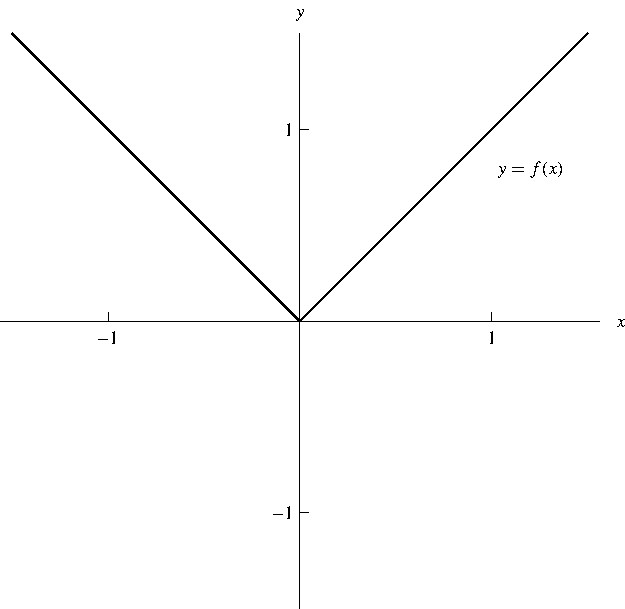
\includegraphics[height=3cm]{derivatives/pictures/03-02-ex5a.pdf}%

\ \only<handout:-2| -30>{%
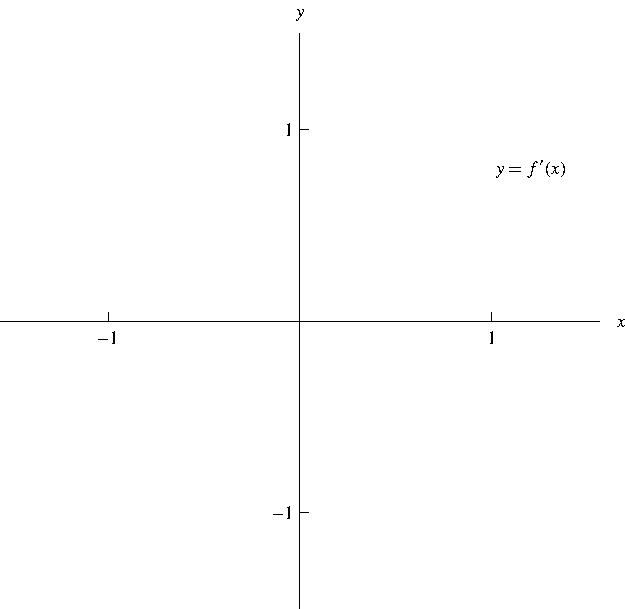
\includegraphics[height=3cm]{derivatives/pictures/03-02-ex5b.pdf}%
}%
\only<handout:3| 31->{%
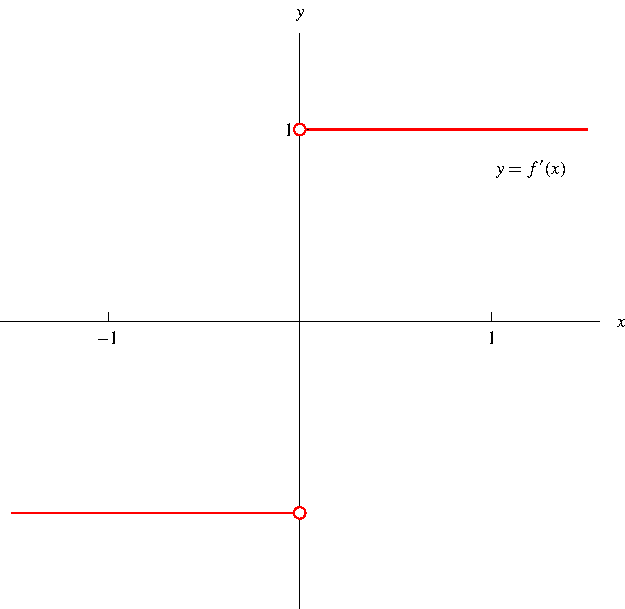
\includegraphics[height=3cm]{derivatives/pictures/03-02-ex5c.pdf}%
}%
\column{.75\textwidth}
\only<handout:1| -10>{%
\begin{itemize}
\item<2->  Suppose $x > 0$.
\item<3-| alert@7>  Then $|x| = x$.
\item<4->  Pick $h$ small so that $x + h > 0$.
\item<5-| alert@7>  Then $|x + h| = x+h$.
\end{itemize}
\abovedisplayskip=0pt
\belowdisplayskip=0pt
\begin{align*}
\uncover<6->{f'(x)}%
 & \uncover<6->{ = } %
\uncover<6->{\lim_{h\rightarrow 0} \frac{|x+h|-|x|}{h}}\\%
 & \uncover<7->{ = } %
\uncover<7->{\lim_{h\rightarrow 0} \frac{(x+h)-x}{h}}\\%
 & \uncover<8->{ = } %
\uncover<8->{\lim_{h\rightarrow 0} \frac{h}{h}}\uncover<9->{ = 1}%
\end{align*}
\uncover<10->{%
Therefore $f$ is differentiable for any $x > 0$.
}%
}%

\only<handout:2| 11-19>{%
\begin{itemize}
\item<11->  Suppose $x < 0$.
\item<12-| alert@16>  Then $|x| = -x$.
\item<13->  Pick $h$ small so that $x + h < 0$.
\item<14-| alert@16>  Then $|x + h| = -(x+h)$.
\end{itemize}
\abovedisplayskip=0pt
\belowdisplayskip=0pt
\begin{align*}
\uncover<15->{f'(x)}%
 & \uncover<15->{ = } %
\uncover<15->{\lim_{h\rightarrow 0} \frac{|x+h|-|x|}{h}}\\%
 & \uncover<16->{ = } %
\uncover<16->{\lim_{h\rightarrow 0} \frac{-(x+h)+x}{h}}\\%
 & \uncover<17->{ = } %
\uncover<17->{\lim_{h\rightarrow 0} \frac{-h}{h}}\uncover<18->{ = -1}%
\end{align*}
\uncover<19->{%
Therefore $f$ is differentiable for any $x < 0$.
}%
}%


\only<handout:3| 20->{%
If $f'(0)$ exists, then 
\[
f'(0) = \lim_{h\rightarrow 0}\frac{f(0+h) - f(0)}{h} = \lim_{h\rightarrow 0} \frac{|0+h| - |0|}{h}.
\]
\uncover<21->{%
Does this limit exist?
}%
\abovedisplayskip=0pt
\belowdisplayskip=0pt
\[
\uncover<22->{%
\lim_{h\rightarrow 0^{\alert<handout:0| 24>{+}}}\frac{|0+h|-|0|}{h}
}%
\uncover<23->{%
 = \lim_{h\rightarrow 0^{\alert<handout:0| 24>{+}}}\frac{\alert<handout:0| 24>{|h|}}{h}
}%
\uncover<24->{%
 = \lim_{h\rightarrow 0^{\alert<handout:0| 24>{+}}}\frac{\alert<handout:0| 24>{h}}{h}
}%
\uncover<25->{%
 = 1
}%
\]
\abovedisplayskip=0pt
\belowdisplayskip=0pt
\[
\uncover<26->{%
\lim_{h\rightarrow 0^{\alert<handout:0| 28>{-}}}\frac{|0+h|-|0|}{h}
}%
\uncover<27->{%
 = \lim_{h\rightarrow 0^{\alert<handout:0| 28>{-}}}\frac{\alert<handout:0| 28>{|h|}}{h}
}%
\uncover<28->{%
 = \lim_{h\rightarrow 0^{\alert<handout:0| 28>{-}}}\frac{\alert<handout:0| 28>{-h}}{h}
}%
\uncover<29->{%
 = -1
}%
\]
\uncover<30->{%
Therefore $f$ is not differentiable at $0$.
}%
\uncover<31->{%
\abovedisplayskip=0pt
\belowdisplayskip=0pt
\[
f'(x) = \left\{ \begin{array}{rl}
1 & \textrm{ if } x > 0\\
-1 & \textrm{ if } x < 0\\
\end{array}\right.
\]
}%
}%
\end{columns}
\end{example}
\end{frame}
% end module differentiable-ex5

%% begin module product-rule
\begin{frame}
\begin{theorem}[The Product Rule]
If $f$ and $g$ are both differentiable, then
\abovedisplayskip=0pt
\belowdisplayskip=0pt
\[
\alertNoH{20}{ \left(f(x)g(x)\right)' =f'(x) g(x)+ f(x) g'(x)}  .
\]
\end{theorem}
\begin{proof}
\uncover<2->{Let $\alertNoH{ 4,20}{F(x) = f(x)g(x)}$.  Then}
\abovedisplayskip=0pt
\belowdisplayskip=-15pt
\abovedisplayshortskip=0pt
\belowdisplayshortskip=0pt
\begin{align*}
 \uncover<2->{\alertNoH{20}{F'(x)}}  & \uncover<2->{ = } \uncover<3->{\lim_{h\rightarrow 0}\frac{F(x+h)-F(x)}{h}}  \uncover<4->{ = } \uncover<4->{\lim_{h\rightarrow 0}\frac{f(x+h)g(x+h) - f(x)g(x)}{h}}\\
& \uncover<5->{ = }  %
\uncover<5->{\lim_{h\rightarrow 0}\frac{\alertNoH{6}{f(x+h)}\alertNoH{7}{g(x+h)} \alertNoH{ 5}{\alertNoH{7}{-} \alertNoH{6}{f(x+h)}\alertNoH{7}{g(x)} + \alertNoH{9}{f(x+h)}\alertNoH{8}{ g(x)}} \alertNoH{9}{- f(x)}\alertNoH{8}{g(x)}}{\alertNoH{10}{h}}}\\
& \uncover<6->{ = }  %
\uncover<6->{\lim_{h\rightarrow 0}\left( \alertNoH{6}{ f(x+h)} \frac{\alertNoH{7}{g(x+h)- g(x)}}{\alertNoH{10}{h}} + \alertNoH{8}{g(x)}\frac{\alertNoH{9}{f(x+h)- f(x)}}{\alertNoH{10}{h}}\right)}\\
& \uncover<11->{ = }  %
\uncover<11->{\alertNoH{ 12-13}{\lim_{h\rightarrow 0}f(x+h)} \alertNoH{ 14-15}{\cdot \lim_{h\rightarrow 0}\frac{g(x+h) - g(x)}{h}}}\\
& \qquad \uncover<11->{ + \alertNoH{ 16-17}{\lim_{h\rightarrow 0}g(x)}\alertNoH{ 18-19}{\cdot\lim_{h\rightarrow 0}\frac{f(x+h)- f(x)}{h}} } %
\alertNoH{20}{ \uncover<12->{ = }  \fcAnswerUncover{12}{13}{f(x)}\fcAnswerUncover{12}{ 15}{g'(x)}  + \fcAnswerUncover{12}{ 17}{g(x)} \fcAnswerUncover{12}{ 19}{f'(x) } }  \uncover<20->{\mbox{\qedhere}}
\end{align*}
\end{proof}
\end{frame}
% end module product-rule

% begin module quotient-rule
\begin{frame}
\begin{theorem}[The Quotient Rule]
If $f$ and $g$ are differentiable and $g(x)\neq 0$, then
\[
\renewcommand{\arraystretch}{2}
\begin{array}{rcl l|l}
\displaystyle \alertNoH{2}{ \frac{\diff}{\diff x} \left( \frac{f(x)}{g(x)}\right)} &=&\displaystyle  \frac{\alertNoH{3}{\frac{\diff}{\diff x} \left( f(x)\right)} g(x)- f(x) \alertNoH{4}{\frac{\diff}{\diff x}\left(g(x)\right)}}{\left(g(x)\right)^2} &&\text{(\alertNoH{2,3,4}{Leibniz notation})}\\
\uncover<2->{ \displaystyle \alertNoH{2}{\left( \frac{f(x)}{g(x)} \right)'} &=&\displaystyle  \frac{ \alertNoH{3}{f'(x)} g(x)- f(x)\alertNoH{4}{ g'(x)}}{\left(g(x)\right)^2}&& \alertNoH{2,3,4}{'\text{ notation}}}\\
\uncover<5->{ \displaystyle \left( \frac{f}{g} \right)' &=&\displaystyle  \frac{ f' g- f g'}{g^2}&& \alertNoH{5}{\text{abbreviated}}} \\
\end{array}
\]
\end{theorem}
\begin{itemize}
\item<6-> The proof of the Quotient Rule is similar to the proof of the Product Rule. 
\item<7-> There is an alternative algebraic proof via the Product Rule, the Power Rule and the (not yet studied) Chain Rule.
\end{itemize}



\end{frame}
% end module quotient-rule

% end lecture

\end{document}
